\documentclass{beamer}
\usepackage[utf8]{inputenc}

\usetheme{Madrid}
\usecolortheme{default}
\usepackage{amsmath,amssymb,amsfonts,amsthm}
\usepackage{txfonts}
\usepackage{tkz-euclide}
\usepackage{listings}
\usepackage{adjustbox}
\usepackage{array}
\usepackage{tabularx}
\usepackage{gvv}
\usepackage{lmodern}
\usepackage{circuitikz}
\usepackage{tikz}
\usepackage{graphicx}
\usepackage{mathtools}

\setbeamertemplate{page number in head/foot}[totalframenumber]

\usepackage{tcolorbox}
\tcbuselibrary{minted,breakable,xparse,skins}



\definecolor{bg}{gray}{0.95}
\DeclareTCBListing{mintedbox}{O{}m!O{}}{%
  breakable=true,
  listing engine=minted,
  listing only,
  minted language=#2,
  minted style=default,
  minted options={%
    linenos,
    gobble=0,
    breaklines=true,
    breakafter=,,
    fontsize=\small,
    numbersep=8pt,
    #1},
  boxsep=0pt,
  left skip=0pt,
  right skip=0pt,
  left=25pt,
  right=0pt,
  top=3pt,
  bottom=3pt,
  arc=5pt,
  leftrule=0pt,
  rightrule=0pt,
  bottomrule=2pt,
  toprule=2pt,
  colback=bg,
  colframe=orange!70,
  enhanced,
  overlay={%
    \begin{tcbclipinterior}
    \fill[orange!20!white] (frame.south west) rectangle ([xshift=20pt]frame.north west);
    \end{tcbclipinterior}},
  #3,
}
\lstset{
    language=C,
    basicstyle=\ttfamily\small,
    keywordstyle=\color{blue},
    stringstyle=\color{orange},
    commentstyle=\color{green!60!black},
    numbers=left,
    numberstyle=\tiny\color{gray},
    breaklines=true,
    showstringspaces=false,
}
\title{12.163}
\date{4th October, 2025}
\author{Puni Aditya - EE25BTECH11046}

\begin{document}

\frame{\titlepage}
\begin{frame}{Question}
The geometric transformation specified by
\begin{align*}
    \myvec{X' & Y' & 1} = \myvec{X & Y & 1} \myvec{0.5 & 0 & 0 \\ 0 & 0.25 & 0 \\ 1 & 2 & 1}
\end{align*}
in a 2D CAD system represents
\begin{enumerate}
    \item Scaling and Translation
    \item Scaling and Rotation
    \item Rotation and Translation
    \item Rotation
\end{enumerate}
\end{frame}

\begin{frame}{Theoretical Solution}
A 2D affine transformation is of the form $\vec{x}'^\top = \vec{x}^\top\vec{T}$, where the transformation matrix is
\begin{align*}
    \vec{T} = \myvec{
        \vec{A} & \vec{0} \\
        \vec{t}^\top & 1
    }
\end{align*}
The given transformation matrix is:
\begin{align}
    \vec{T} = \myvec{0.5 & 0 & 0 \\ 0 & 0.25 & 0 \\ 1 & 2 & 1}
\end{align}
\end{frame}

\begin{frame}{Theoretical Solution}
From this, we identify the linear transformation matrix $\vec{A}$ and the translation vector $\vec{t}$.
\begin{align}
    \vec{A} = \myvec{0.5 & 0 \\ 0 & 0.25}, \quad \vec{t} = \myvec{1 \\ 2}
\end{align}
Since $\vec{A}$ is a diagonal matrix and not a multiple of the identity, it represents a non-uniform scaling. Since $\vec{t} \neq \vec{0}$, there is a translation.
\end{frame}

\begin{frame}{Theoretical Solution}
A pure rotation requires the linear part $\vec{A}$ to be an orthogonal matrix, where $\vec{A}\vec{A}^\top = \vec{I}$. We check this condition:
\begin{align}
    \vec{A}\vec{A}^\top = \myvec{0.5 & 0 \\ 0 & 0.25}\myvec{0.5 & 0 \\ 0 & 0.25} = \myvec{0.25 & 0 \\ 0 & 0.0625} \neq \vec{I}
\end{align}
Since $\vec{A}$ is not orthogonal, the transformation is not a rotation.
\end{frame}

\begin{frame}{Example}
Applying the transformation to the point $\myvec{1 \\ 1}$. In homogeneous coordinates, $\vec{x}^\top = \myvec{1 & 1 & 1}$.
\begin{align*}
    \vec{x}'^\top &= \myvec{1 & 1 & 1} \myvec{0.5 & 0 & 0 \\ 0 & 0.25 & 0 \\ 1 & 2 & 1} \\
    &= \myvec{1.5 & 2.25 & 1}
\end{align*}
The point $\myvec{1 \\ 1}$ is transformed to $\myvec{1.5 \\ 2.25}$, demonstrating both scaling and translation.

The correct option is \textbf{1) Scaling and Translation}.
\end{frame}

\begin{frame}{Plot}
\begin{figure}
    \centering
    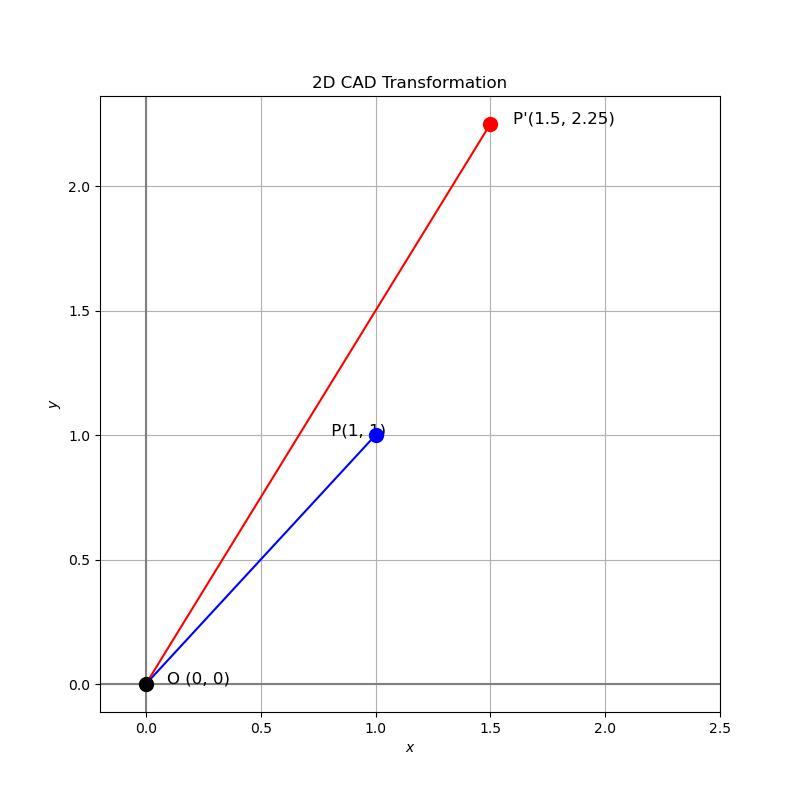
\includegraphics[width=0.5\columnwidth]{../figs/plot_p.jpg}
    \caption{Plot}
    \label{fig:fig}
\end{figure}
\end{frame}

\end{document}
